% Beamer slide template prepared by Tom Clark <tom.clark@op.ac.nz>
% Otago Polytechnic
% Dec 2012

\documentclass[10pt]{beamer}
\usetheme{Dunedin}
\usepackage{graphicx}
\usepackage{fancyvrb}

\newcommand\codeHighlight[1]{\textcolor[rgb]{1,0,0}{\textbf{#1}}}

\title{Network Sockets 2}

\author[IN608]{Intermediate Application Development}
\institute[Otago Polytechnic]{
  Otago Polytechnic \\
  Dunedin, New Zealand \\
  Kaiako: Tom Clark
}
\date{}
\begin{document}

%----------- titlepage ----------------------------------------------%
\begin{frame}[plain]
  \titlepage
\end{frame}

%----------- slide --------------------------------------------------%
\begin{frame}
  \frametitle{Introduction}
  
  Last time we saw how to get network sockets working from the client and
  the server side. Our basic implementations had a lot of problems. One of them
  was that our server could only respond to one client at a time. We overcame that 
  by using selectors to multiplex over our client sockets.
  
  \vspace{5mm}
  This time we will see how to overcome another big problem.  
  \end{frame}

%----------- slide --------------------------------------------------%
\begin{frame}
  \frametitle{Network model}
  
  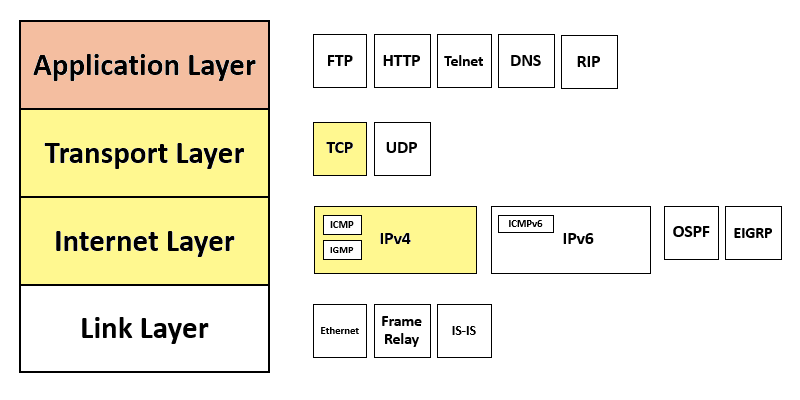
\includegraphics[width=8cm]{tcp-ip.png}
  
  {\tiny image: Michel Bakni (\url{https://www.wikidata.org/wiki/Q81411358})}  
  \end{frame}

%----------- slide --------------------------------------------------%
\begin{frame}[fragile]
  \frametitle{The problem}
  
  \begin{Verbatim}[commandchars=\\\{\}]
  # Server:                                                                                                       
  import socket                                           
  s = socket.socket(socket.AF_INET, socket.SOCK_STREAM)  
  s.bind(('127.0.0.1', 65432))                          
  s.listen()                                             
  conn, addr = s.accept()                                
  data = \codeHighlight{conn.recv(1024)}                                                                                                                
 \end{Verbatim} 
 
 \vspace{5mm}
 What if we want to send and receive longer messages?
   
\end{frame}

%----------- slide --------------------------------------------------%
\begin{frame}
  \frametitle{Two options}
  
   
  \begin{enumerate}
    \item Require that our application uses fixed-length messages.
    \item Make the messages indicate how long they are.
  \end{enumerate}
  
  
    
  \end{frame}

%----------- slide --------------------------------------------------%
\begin{frame}
  \frametitle{A simple header}
  
  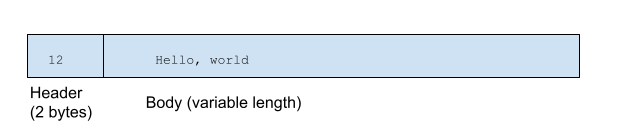
\includegraphics[width=8cm]{message.png}
  
 
  \end{frame}

%----------- slide --------------------------------------------------%
\begin{frame}
  \frametitle{Warning}
  
  We're heading into territory where we're manipulating things byte-by-byte.
  None of this is rocket science, but there are a lot of details to worry 
  about.
  
 
  \end{frame}

%----------- slide --------------------------------------------------%
\begin{frame}[fragile]
  \frametitle{Message: send}
  
  \begin{verbatim}
  import struct
  
  def send(txt, sock):
    msgbody = bytes(txt.encode('utf-8'))
    msglen = len(msgbody)
    header = struct.pack('>H', msglen) # 2-byte unsigned int
    message = header + msgbody
    sock.sendall(message)
  
             
  \end{verbatim} 
   
\end{frame}

%----------- slide --------------------------------------------------%
\begin{frame}[fragile]
  \frametitle{Message: receive}
  
  \begin{verbatim}
    def receive(sock):
        data = b''
        while len(data) < 2:
            data = sock.recv(4)
        body_length  = struct.unpack('>H', data[:2])[0]
        print(body_length)
        data = data[2:]
        while len(data) < body_length:
            data += sock.recv(4)
        return data.decode('utf-8')  \end{verbatim} 
   

(Yes, calling \texttt{sock.recv(4)} is a bit silly, but it demonstrates our process with
small messages.)
\end{frame}
%----------- slide --------------------------------------------------%
\begin{frame}
  \frametitle{Programming Activity}
  
  \begin{enumerate}
    \item Pull the course materials repo.
    \item Create a new branch, \texttt{20-practical} in your practicals repo.
    \item Copy the subdirectory, \texttt{20-practical} from the class materials into your repo.
    \item See the README for directions.
    \item We will discuss results in 30ish minutes.
  \end{enumerate}      
\end{frame}
  
%----------- slide --------------------------------------------------%
\begin{frame}
  \frametitle{More Cowbell}
  
  We now have a de facto ``application protocol'' that lets us send and 
  receive utf-8 strings of up to about 64kb length.  We can do better.
  
  \vspace{5mm}
  If we could define a larger header with multiple fields, then we could 
  attach more metadata to our application messages.
      
\end{frame}

%----------- slide --------------------------------------------------%
\begin{frame}[fragile]
  \frametitle{Header format}
  
  It's our application, so we can do anything we want with the header. We
  probably want it to be text. Using JSON makes it easy to parse.
  \begin{verbatim}
  
    {
     'Context-type': 'text/plain',
     'Content-encoding': 'utf-8',
     'Content-length': 46
    }
  \end{verbatim}   
  
  We put a header like this before our body. An application can use this
  to determine how to process the body.
     
\end{frame}

%----------- slide --------------------------------------------------%
\begin{frame}
  \frametitle{A full header}
  
  Now we have a new problem. How long is the header? But we already solved this.
  
  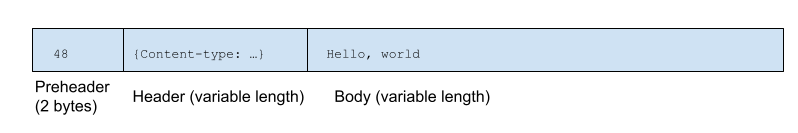
\includegraphics[width=8cm]{message2.png}
  
  The preheader tells us how long the header is. The header tells us how
  long the body is. 
 
  \end{frame}


%----------- slide --------------------------------------------------%
\begin{frame}
  \frametitle{Writing a message}
  
  The process of writing a message is
  \begin{enumerate}
    \item Get your message body and convert it to bytes.
    \item Prepare your header, now that you know how long the body is, and convert it to bytes.
    \item Prepare your preheader with the length of your header.
    \item Assemble the three parts.
    \item Send the message.
  \end{enumerate}      
\end{frame}
%----------- slide --------------------------------------------------%
\begin{frame}
  \frametitle{Reading a message}
  
  The process of reading a message is
  \begin{enumerate}
    \item Get at least two bytes in an input buffer.
    \item Process the preheader and remove it from the buffer.
    \item Collect enough bytes in the buffer to hold the header.
    \item Process the header and remove its bytes from the buffer.
    \item Collect the bytes for the body and process it.
    \item Send the message.
  \end{enumerate}
  
  At this point we probably have enough structure to warrant a \texttt{Message} class.      
\end{frame}


\end{document}
